\documentclass[tikz,border=8pt]{standalone}
\usetikzlibrary{arrows.meta,positioning,shapes.geometric,fit,calc}
\definecolor{navy}{HTML}{213A5B}
\definecolor{blue}{HTML}{3977A8}
\definecolor{teal}{HTML}{27826F}
\definecolor{orange}{HTML}{C56A36}
\definecolor{violet}{HTML}{7656A5}
\definecolor{paleBlue}{HTML}{EAF2F8}
\definecolor{paleTeal}{HTML}{E9F4F0}
\definecolor{paleOrange}{HTML}{FCF0E7}
\definecolor{paleViolet}{HTML}{F1ECF8}
\tikzset{
  data/.style={draw=blue!75!black,fill=paleBlue,rounded corners=1.5mm,
    line width=.9pt,align=center,text width=2.8cm,minimum height=.78cm,
    inner sep=4pt,font=\scriptsize},
  train/.style={draw=teal!80!black,fill=paleTeal,rounded corners=1.5mm,
    line width=.9pt,align=center,text width=2.45cm,minimum height=.72cm,
    inner sep=4pt,font=\scriptsize},
  model/.style={draw=orange!85!black,fill=paleOrange,rounded corners=1.5mm,
    line width=.9pt,align=center,text width=2.65cm,minimum height=.78cm,
    inner sep=4pt,font=\scriptsize},
  result/.style={draw=violet!80!black,fill=paleViolet,rounded corners=1.5mm,
    line width=1pt,align=center,text width=2.65cm,minimum height=.78cm,
    inner sep=4pt,font=\scriptsize},
  decision/.style={diamond,draw=teal!80!black,fill=paleTeal,line width=.9pt,
    aspect=2,align=center,inner sep=2pt,font=\scriptsize},
  laneA/.style={draw=blue!45,fill=blue!4,rounded corners=2mm,line width=.7pt},
  laneB/.style={draw=violet!45,fill=violet!4,rounded corners=2mm,line width=.7pt},
  prep/.style={draw=teal!35,fill=teal!3,rounded corners=2mm,line width=.7pt},
  flow/.style={-{Stealth[length=2mm]},draw=navy,line width=.85pt},
  trainflow/.style={flow,draw=teal!80!black},
  testflow/.style={flow,draw=violet!80!black},
  lab/.style={font=\tiny,fill=white,inner sep=1pt,text=navy,align=center},
  heading/.style={font=\bfseries\small,text=navy}
}
\begin{document}
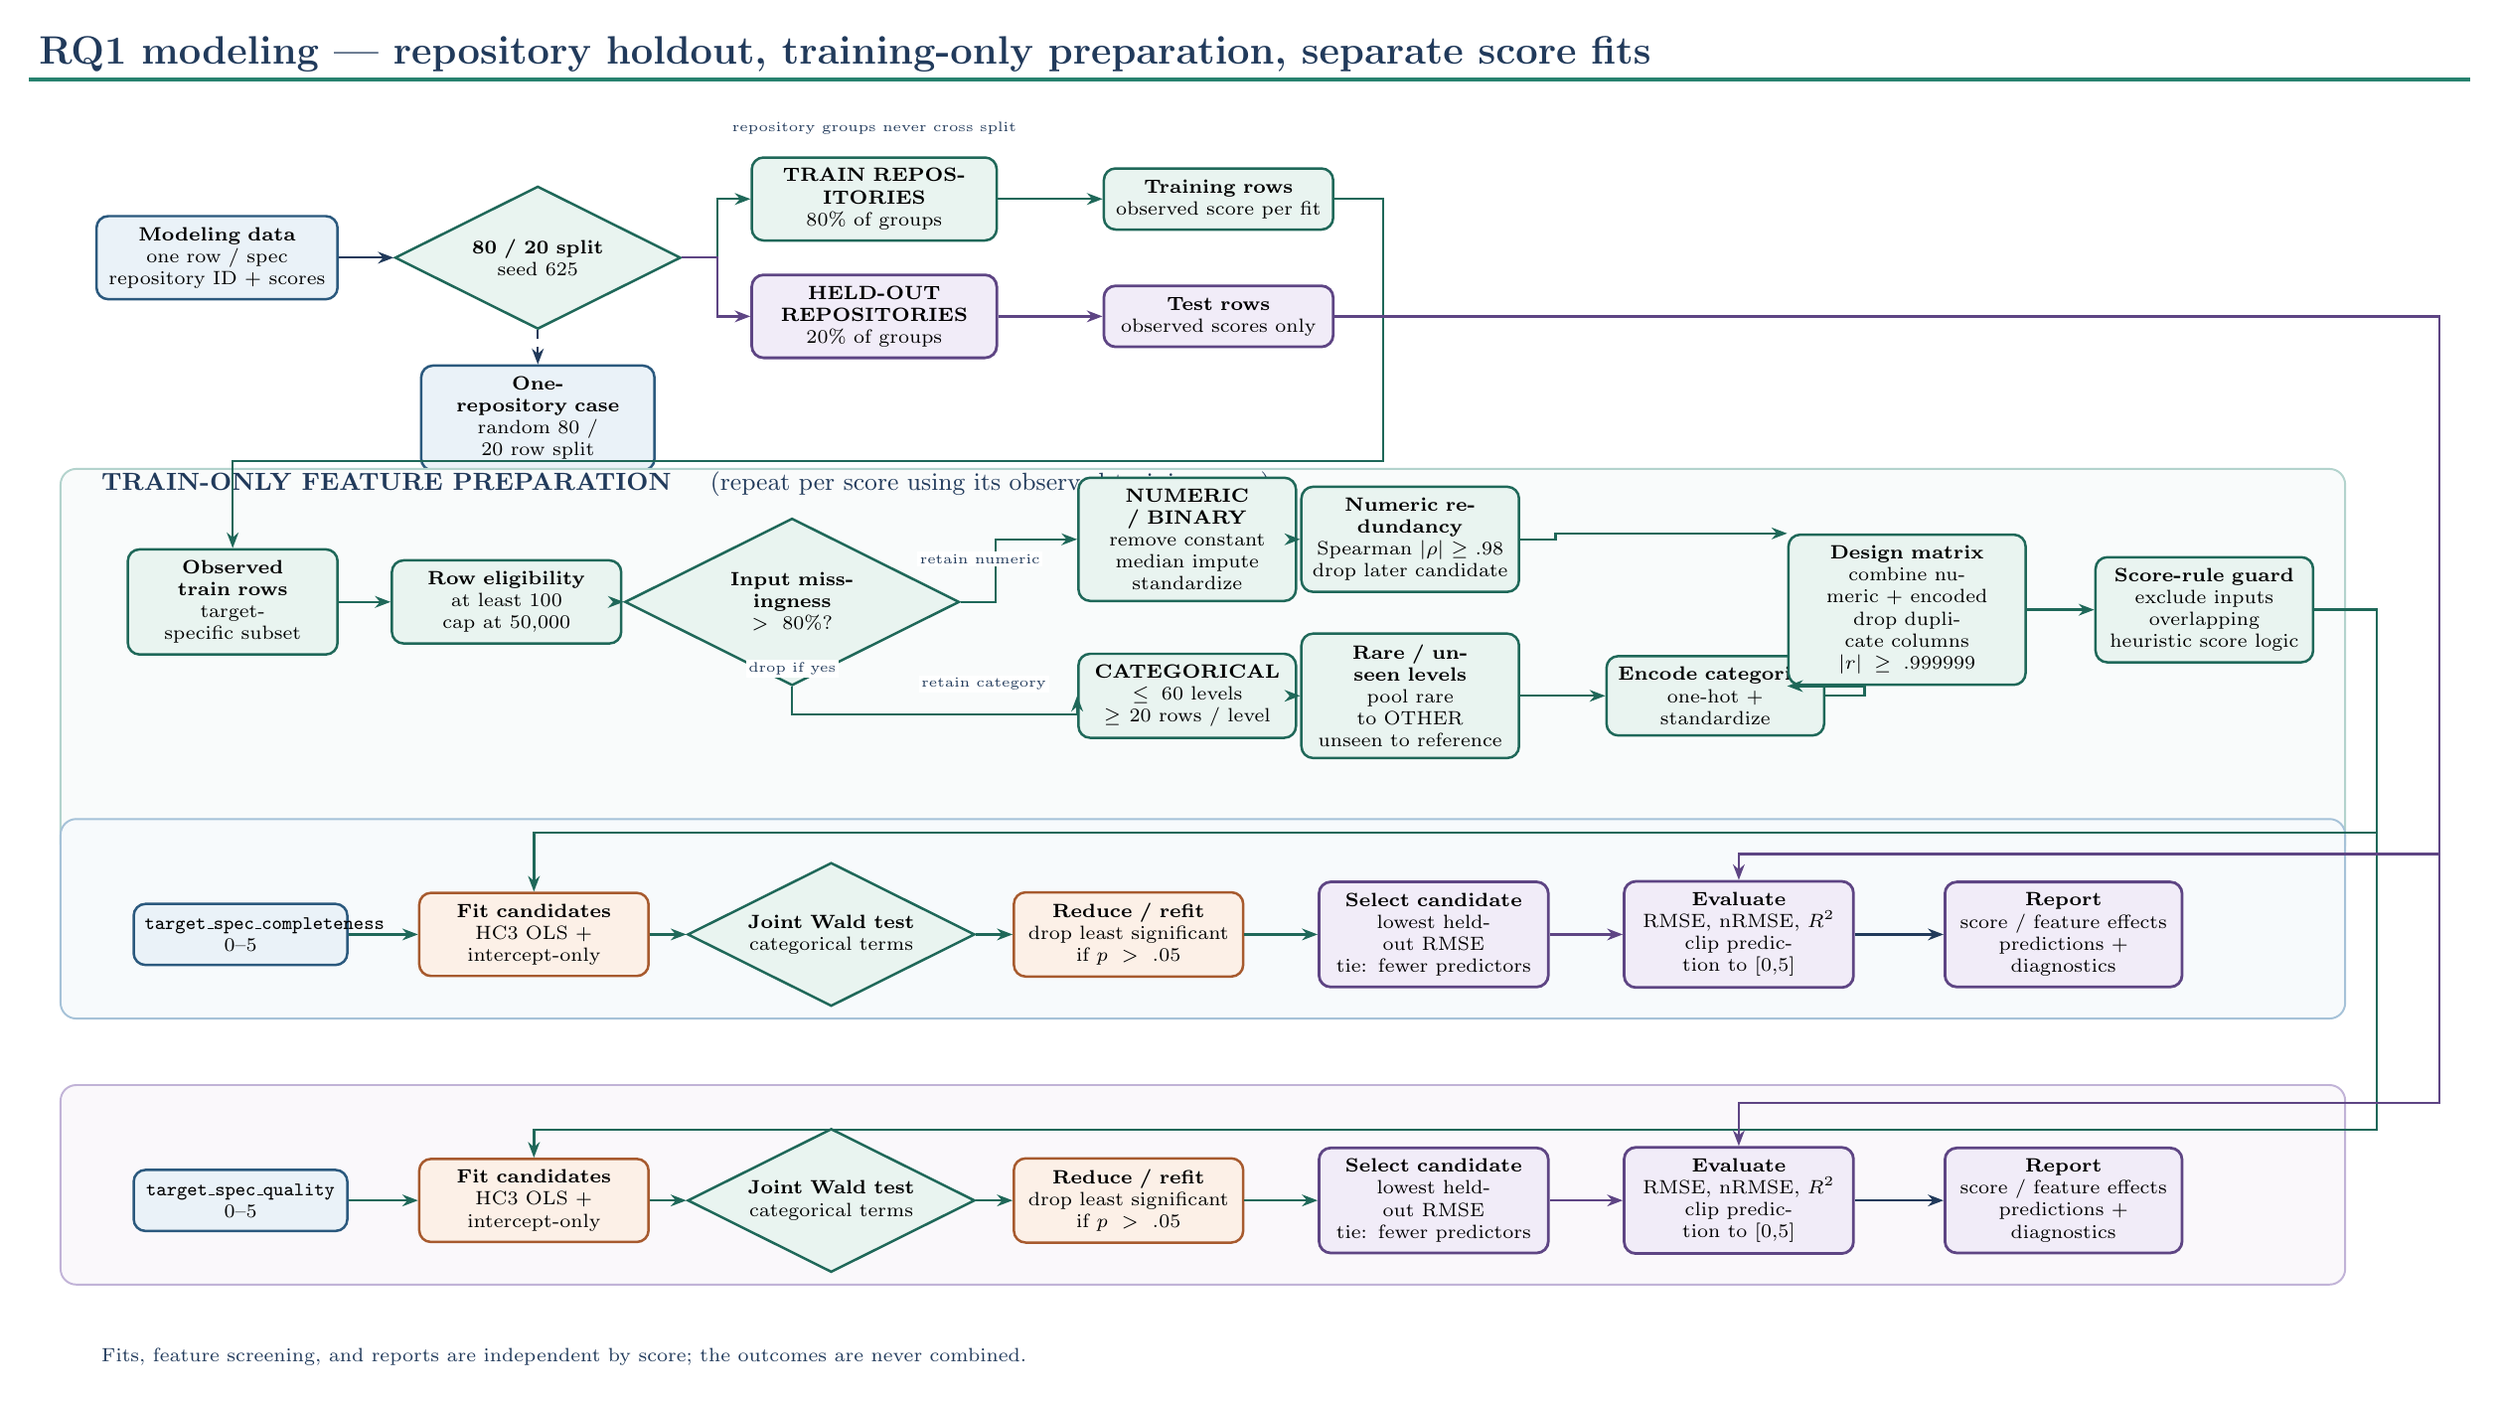
\begin{tikzpicture}[font=\sffamily]
  \node[anchor=west,text=navy,font=\bfseries\Large] at (-15,13)
    {RQ1 modeling | repository holdout, training-only preparation, separate score fits};
  \draw[teal,line width=1.3pt] (-15,12.68) -- (16.2,12.68);

  % Split by repository, not by specification, whenever multiple repositories exist.
  \node[data] (input) at (-12.6,10.4)
    {\textbf{Modeling data}\\one row / spec\\repository ID + scores};
  \node[decision,text width=2.3cm] (split) at (-8.5,10.4)
    {\textbf{80 / 20 split}\\seed 625};
  \node[train,text width=2.85cm] (trainrepos) at (-4.2,11.15)
    {\textbf{TRAIN REPOSITORIES}\\80\% of groups};
  \node[result,text width=2.85cm] (testrepos) at (-4.2,9.65)
    {\textbf{HELD-OUT REPOSITORIES}\\20\% of groups};
  \node[train,text width=2.65cm] (trainset) at (.2,11.15)
    {\textbf{Training rows}\\observed score per fit};
  \node[result,text width=2.65cm] (testset) at (.2,9.65)
    {\textbf{Test rows}\\observed scores only};
  \node[data,text width=2.7cm] (fallback) at (-8.5,8.35)
    {\textbf{One-repository case}\\random 80 / 20 row split};
  \draw[flow] (input) -- (split);
  \draw[trainflow] (split.east) -- ++(.45,0) |- (trainrepos.west);
  \draw[testflow] (split.east) -- ++(.45,0) |- (testrepos.west);
  \draw[trainflow] (trainrepos.east) -- (trainset.west);
  \draw[testflow] (testrepos.east) -- (testset.west);
  \draw[flow,dashed] (split.south) -- (fallback.north);
  \node[lab] at (-4.2,12.05) {repository groups never cross split};

  % Shared visual preparation recipe, executed independently for each score.
  \node[prep,minimum width=29.2cm,minimum height=5.0cm] at (0,5.2) {};
  \node[heading,anchor=west] at (-14.2,7.5)
    {TRAIN-ONLY FEATURE PREPARATION \quad\textnormal{(repeat per score using its observed training rows)}};
  \node[train,text width=2.4cm] (rows) at (-12.4,6.0)
    {\textbf{Observed train rows}\\target-specific subset};
  \node[train,text width=2.65cm] (eligibility) at (-8.9,6.0)
    {\textbf{Row eligibility}\\at least 100\\cap at 50,000};
  \node[decision,text width=2.35cm] (missing) at (-5.25,6.0)
    {\textbf{Input missingness}\\$>80\%$?};
  \node[train,text width=2.5cm] (numeric) at (-.2,6.8)
    {\textbf{NUMERIC / BINARY}\\remove constant\\median impute\\standardize};
  \node[train,text width=2.5cm] (categorical) at (-.2,4.8)
    {\textbf{CATEGORICAL}\\$\leq60$ levels\\$\geq20$ rows / level};
  \node[train,text width=2.5cm] (numericcorr) at (2.65,6.8)
    {\textbf{Numeric redundancy}\\Spearman $|\rho|\geq.98$\\drop later candidate};
  \node[train,text width=2.5cm] (rare) at (2.65,4.8)
    {\textbf{Rare / unseen levels}\\pool rare to OTHER\\unseen to reference};
  \node[train,text width=2.5cm] (encoded) at (6.55,4.8)
    {\textbf{Encode categories}\\one-hot + standardize};
  \node[train,text width=2.75cm] (design) at (9.0,5.9)
    {\textbf{Design matrix}\\combine numeric + encoded\\drop duplicate columns\\$|r|\geq.999999$};
  \node[train,text width=2.5cm] (leakage) at (12.8,5.9)
    {\textbf{Score-rule guard}\\exclude inputs overlapping\\heuristic score logic};

  \draw[trainflow] (trainset.east) -- (2.3,11.15) -- (2.3,7.8)
    -- (-12.4,7.8) -- (rows.north);
  \draw[trainflow] (rows) -- (eligibility);
  \draw[trainflow] (eligibility) -- (missing);
  \draw[trainflow] (missing.east) -- ++(.45,0) |- (numeric.west);
  \draw[trainflow] (missing.south) -- ++(0,-.35) -| (categorical.west);
  \node[lab] at (-2.85,6.55) {retain numeric};
  \node[lab] at (-2.8,4.95) {retain category};
  \node[lab] at (-5.25,5.15) {drop if yes};
  \draw[trainflow] (numeric) -- (numericcorr);
  \draw[trainflow] (categorical) -- (rare);
  \draw[trainflow] (rare) -- (encoded);
  \draw[trainflow] (numericcorr.east) -- ++(.45,0) |- (design.north west);
  \draw[trainflow] (encoded.east) -- ++(.5,0) |- (design.south west);
  \draw[trainflow] (design) -- (leakage);

  % Two distinct score lanes; nothing is combined into a composite outcome.
  \node[laneA,minimum width=29.2cm,minimum height=2.55cm] at (0,1.95) {};
  \node[laneB,minimum width=29.2cm,minimum height=2.55cm] at (0,-1.45) {};
  \node[data,text width=2.45cm] (complete) at (-12.3,1.75)
    {\texttt{target\_spec\_completeness}\\0--5};
  \node[model] (fitA) at (-8.55,1.75)
    {\textbf{Fit candidates}\\HC3 OLS + intercept-only};
  \node[decision,text width=2.25cm] (waldA) at (-4.75,1.75)
    {\textbf{Joint Wald test}\\categorical terms};
  \node[model] (reduceA) at (-.95,1.75)
    {\textbf{Reduce / refit}\\drop least significant\\if $p>.05$};
  \node[result] (selectA) at (2.95,1.75)
    {\textbf{Select candidate}\\lowest held-out RMSE\\tie: fewer predictors};
  \node[result] (evalA) at (6.85,1.75)
    {\textbf{Evaluate}\\RMSE, nRMSE, $R^2$\\clip prediction to [0,5]};
  \node[result,text width=2.75cm] (reportA) at (11.0,1.75)
    {\textbf{Report}\\score / feature effects\\predictions + diagnostics};

  \node[data,text width=2.45cm] (quality) at (-12.3,-1.65)
    {\texttt{target\_spec\_quality}\\0--5};
  \node[model] (fitB) at (-8.55,-1.65)
    {\textbf{Fit candidates}\\HC3 OLS + intercept-only};
  \node[decision,text width=2.25cm] (waldB) at (-4.75,-1.65)
    {\textbf{Joint Wald test}\\categorical terms};
  \node[model] (reduceB) at (-.95,-1.65)
    {\textbf{Reduce / refit}\\drop least significant\\if $p>.05$};
  \node[result] (selectB) at (2.95,-1.65)
    {\textbf{Select candidate}\\lowest held-out RMSE\\tie: fewer predictors};
  \node[result] (evalB) at (6.85,-1.65)
    {\textbf{Evaluate}\\RMSE, nRMSE, $R^2$\\clip prediction to [0,5]};
  \node[result,text width=2.75cm] (reportB) at (11.0,-1.65)
    {\textbf{Report}\\score / feature effects\\predictions + diagnostics};

  \draw[trainflow] (leakage.east) -- ++(.45,0) -- (15.0,5.9)
    -- (15.0,3.05) -- (-8.55,3.05) -- (fitA.north);
  \draw[trainflow] (15.0,5.9) -- (15.0,-.75) -- (-8.55,-.75) -- (fitB.north);
  \draw[trainflow] (complete) -- (fitA);
  \draw[trainflow] (fitA) -- (waldA);
  \draw[trainflow] (waldA) -- (reduceA);
  \draw[trainflow] (reduceA) -- (selectA);
  \draw[testflow] (selectA) -- (evalA);
  \draw[flow] (evalA) -- (reportA);

  \draw[trainflow] (quality) -- (fitB);
  \draw[trainflow] (fitB) -- (waldB);
  \draw[trainflow] (waldB) -- (reduceB);
  \draw[trainflow] (reduceB) -- (selectB);
  \draw[testflow] (selectB) -- (evalB);
  \draw[flow] (evalB) -- (reportB);

  % Held-out outcomes are used for candidate comparison and test reporting.
  \draw[testflow] (testset.east) -- ++(1.0,0) -- (15.8,9.65)
    -- (15.8,2.78) -- (6.85,2.78) -- (evalA.north);
  \draw[testflow] (15.8,2.78) -- (15.8,-.4) -- (6.85,-.4) -- (evalB.north);

  \node[anchor=west,font=\scriptsize,text=navy] at (-14.2,-3.65)
    {Fits, feature screening, and reports are independent by score; the outcomes are never combined.};
\end{tikzpicture}
\end{document}
